%%%%%%%%%%%%%%%%%%%%%%%%%%%%%%%%%%%%%%%%%%%%%%%%%%%%%%%%%%%%%%%%%%%%%%%%%
%
% File: Model.tex
%
% Purpose: Top level document for Model.  Should not need to be edited.
%
%%%%%%%%%%%%%%%%%%%%%%%%%%%%%%%%%%%%%%%%%%%%%%%%%%%%%%%%%%%%%%%%%%%%%%%%%

\newcommand\documentHistory{
{\bf Author} & {\bf Date} & {\bf Description} \\ \hline \hline
\ModelAuthor & \ModelAuthDate & Initial Version \\ \hline
}


\documentclass[twoside,11pt,titlepage]{report}

%
% Bring in the common page setup
%
\usepackage{dynenv}

%
% Bring in the model-specific commands
%
\usepackage{aerodynamics}

%
% Bring in the graphics environment
%
\usepackage{graphicx}

% use better float package
\usepackage{float}

% use equation package stuff
\usepackage{amsmath, amsthm, amssymb}

%
% Bring in the hyper ref environment
%
\usepackage[colorlinks,plainpages=false]{hyperref}
%  keywords for pdfkeywords are separated by commas
\hypersetup{
   pdftitle={\aerodynamicsDesc},
   pdfauthor={\ModelAuthor},
   pdfkeywords={\ModelKeywords},
   pdfsubject={\aerodynamicsDesc}}

\begin{document}

%%%%%%%%%%%%%%%%%%%%%%%%%%%%%%%%%%%
% Front matter
%%%%%%%%%%%%%%%%%%%%%%%%%%%%%%%%%%%
\pagenumbering{roman}

\docid{models/interactions/aerodynamics}
\docrev{1.2}
\date{\RELEASEMONTH\ \RELEASEYEAR}
\modelname{\aerodynamicsDesc}
\doctype{}
\author{\ModelAuthor}
\managers{
  Robert O. Shelton \\ Project Manager \\
  Michael T. Red \\ Simulation and Graphics Branch Chief \\
  R. Matt Ondler \\ Software, Robotics, and Simulation Division Chief}
\pdfbookmark{Title Page}{titlepage}
\makeDynenvTitlepage

\pdfbookmark{Abstract}{abstract}
%%%%%%%%%%%%%%%%%%%%%%%%%%%%%%%%%%%%%%%%%%%%%%%%%%%%%%%%%%%%%%%%%%%%%%%%
%
% Purpose:
%
%  
%
%%%%%%%%%%%%%%%%%%%%%%%%%%%%%%%%%%%%%%%%%%%%%%%%%%%%%%%%%%%%%%%%%%%%%%%%%

\begin{abstract}

The \aerodynamicsDesc\ computes the forces and torques that model the effects of
aerodynamics on a vehicle.  These forces and torques are summed into
the forces and torques that model the overall vehicle dynamics.  These
models are used to characterize the affects of aerodynamics on a vehicle's
trajectory.  The \aerodynamicsDesc\ consists of two drag modeling options.
There is a simple drag model of using the coefficient of drag or the
ballistic coefficient (also known as the ballistic number) method.
A composite plate model with surfaces that include accommodation factors
for specular, diffuse or mixed reflections (mixed here means a
combination of specular and diffuse).

Additionally, an extensible framework for the addition of new methods of
calculating drag has been implemented, giving flexibility to the end
user of the \JEODid\ package.

\end{abstract}


\pdfbookmark{Contents}{contents}
\tableofcontents
\vfill

\pagebreak

%%%%%%%%%%%%%%%%%%%%%%%%%%%%%%%%%%%
% Main Document Body
%%%%%%%%%%%%%%%%%%%%%%%%%%%%%%%%%%%
\pagenumbering{arabic}

%%% For a simple document make a copy of Chapters.tex and use this format
%%% use of aerodynamicsChapters vs ModelChapters is solely for the purpose of
%%% combatability with the copy_templates.csh script.
\setcounter{chapter}{0}

%----------------------------------
\chapter{Introduction}\hyperdef{part}{intro}{}\label{ch:intro}
%----------------------------------


\section{Model Description}
Atmospheric force is the largest non-gravitational perturbation acting on
spacecraft in low Earth orbit.  Accurate modeling of aerodynamic forces
presents three difficulties: the physical properties of the atmosphere
are not known with high accuracy, the modeling requires knowledge
of the interactions of neutral gas with spacecraft surfaces, and the requirement
of higher fidelity, non-spherical representations of a vehicle.
The dominant atmosphere force acting is called drag and is directed
opposite to the velocity of the vehicle motion.  When the line of incidence
of the aerodynamic drag is not through the center of mass there will be a
torque.  Aerodynamic torques result from the force at the incidence point of
atmospheric drag on the moment arm defined by the distance between
the center of pressure and the center of mass. On-orbit aerodynamics is modeled
in JEOD as simple drag and as free molecular drag.  In addition a further
refinement may be made by modeling the way a surface in the thermosphere
accommodates the impinging atmospheric molecules.

Additionally, this model provides an extensible framework for the addition of
new methods of calculating aerodynamic drag on a vehicle, utilizing both
the \aerodynamicsDesc\ as well as the JEOD Surface Model utility
\cite{dynenv:SURFACEMODEL}.

\section{Document History}
%%% Status of this and only this document.  Any date should be relevant to when
%%% this document was last updated and mention the reason (release, bug fix, etc.)
%%% Mention previous history aka JEOD 1.4-5 heritage in this section.
%%% Mention that JEOD.pdf is the parent document.

\begin{tabular}{||l|l|l|l|} \hline
\DocumentChangeHistory
\end{tabular}

This document derives heavily from it's prececessor,
JSC Engineering Orbital Dynamics On-Orbit Aerodynamics Models
released with JEOD v1.5.2.

The following document is parent to this document:
\begin{itemize}
\item{\href{file:\JEODHOME/docs/JEOD.pdf}
           {\em JSC Engineering Orbital Dynamics}}
\cite{dynenv:JEOD}
\end{itemize}

\section{Document Organization}
This document is formatted in accordance with the
NASA Software Engineering Requirements Standard~\cite{NASA:SWE}
and is organized into the following chapters:

\begin{description}
%% longer chapter descriptions, more information.

\item[Chapter 1: Introduction] -
This introduction contains three sections: description of model, document history, and organization.
The first section provides the introduction to the \aerodynamicsDesc\ and its reason
for existence.  It also contains a brief description of the interconnections with other models, and
references to any supporting documents.  The second section displays the history of this document which includes
author, date, and reason for each revision; it also lists the document that is parent to this one.  The final
section contains a description of how the document is organized.

\item[Chapter 2: Product Requirements] -
Describes requirements for the \aerodynamicsDesc.

\item[Chapter 3: Product Specification] -
Describes the underlying theory, architecture, and design of the \aerodynamicsDesc\ in detail.  It is organized in
three sections: Conceptual Design, Mathematical Formulations, and Detailed Design.

\item[Chapter 4: User Guide] -
Describes how to use the \aerodynamicsDesc\ in a Trick simulation.  It is broken into three sections to represent the JEOD
defined user types: Analysts or users of simulations (Analysis), Integrators or developers of simulations (Integration),
and Model Extenders (Extension).

\item[Chapter 5: Verification and Validation] -
Contains \aerodynamicsDesc\ verification and validation procedures and results.

\end{description}

%----------------------------------
\chapter{Product Requirements}\hyperdef{part}{reqt}{}\label{ch:reqt}
%----------------------------------

This chapter will describe the requirements for the \aerodynamicsDesc.

\requirement{Top-level requirement}
\label{reqt:toplevel}
\begin{description}
\item[Requirement:]\ \newline
  This model shall meet the JEOD project requirements specified in
  the \JEODid\
  \hyperref{file:\JEODHOME/docs/JEOD.pdf}{part1}{reqt}{ top-level
  document}.
\item[Rationale:]\ \newline
  This model shall, at a minimum,  meet all external and internal requirements
  applied to the \JEODid\ release.
\item[Verification:]\ \newline
     Inspection
\end{description}

%%% Format for the model Requirements is open.  It should include requirements for this model
%%% only and use requirment tags like the one below.
%\requirement{...}
%\label{reqt:...}
%\begin{description}
%  \item[...]\ \newline
%    The documentation for the model shall include
%
%    \subrequirement{}
%    \label{reqt:...}
%      Software requirements specification.
%
%    ...
%
%  \item[title]\ \newline
%    text
%
%  ...
%
%\end{description}
\section{Data Requirements}\label{sec:data_reqts}
This section identifies requirements on the data represented by the \aerodynamicsDesc.
These as-built requirements are based on the \aerodynamicsDesc\ data definition header files.

\requirement{Aerodynamic Data}
\label{reqt:AD}
\begin{description}
  \item[Requirement:]\ \newline
    \subrequirement{Drag Modeling Data}\label{reqt:DAD} -
      \aerodynamicsDesc\ shall consist of
\begin{itemize}
\item a model of simple drag ,
\item free molecular flow drag,
\item a method of representing the aerodynamic characteristics of a complex body with a composite of simple surfaces.
\end{itemize}

The modeling shall produce the forces and
      torques on a vehicle as a function of its translational and
      rotational state. The \aerodynamicsDesc\ will provide the input selection
      of ballistic coefficient (BC), coefficient of drag (CD), under
      Newtonian flow and Free Molecular Flow conditions. Free Molecular
      Flow will provide the modeling of specular and diffuse reflection or
      a combination thereof. If not using BC or CD a complex vehicle may
      be modeled using a set of flat plates such that the sum approximates
      the overall drag characteristics of the vehicle. The output of the
      \aerodynamicsDesc\ will be the force and moments due to drag in the structural
frame of the vehicle.
\end{description}

\section{Functional Requirements}\label{sec:func_reqts}
This section identifies requirements on the functional capabilities
provided by the \aerodynamicsDesc.  These as-built requirements are based on the
\aerodynamicsDesc\ source files.

\requirement{On Orbit Drag Modeling}
\label{reqt:drag}
\begin{description}
  \item[Requirement:]\ \newline
   The \aerodynamicsDesc\ shall model aerodynamic drag on a surface, such that
    forces and torques are produced.
    Vehicle area and atmospheric density will be inputs to the modeling.
    The drag modeling shall include:
    \subrequirement{Simple Drag}\label{reqt:sd} -
      The \aerodynamicsDesc\ shall provide the user with the capability to choose
      either a coefficient of drag or a ballistic number to model vehicle
      drag. In addition a simple option for a constant atmospheric density
      will be available.
    \subrequirement{Approximate Free Molecular Flow}\label{reqt:AFM} -
      The \aerodynamicsDesc\ shall provide the user with the capability to choose
      an approximate computation of free molecular drag flow allowing three
      conditional modes of expression. One will be computation of free
      molecular flow using specular reflection. One will be computation of
      free molecular flow using diffuse reflection. One will be computation
      of free molecular flow using a combination of specular and diffuse
      reflection.
    \subrequirement{Free Molecular Flow}\label{reqt:FMF} -
      The \aerodynamicsDesc\ shall provide the user with the capability to choose
      an approximate computation of free molecular drag flow allowing two
      conditional modes of expression. One will be the computation of free
      molecular flow using specular reflection and diffuse reflection by
      specifying the fraction of each. The second will be
      the computation of flow using normal and tangential reflection by
      specifying the fraction of each.
    \subrequirement{Aerodynamic Surfaces}\label{reqt:AS} -
      The \aerodynamicsDesc\ shall provide the ability to represent the forces and
      torques acting on the vehicle by using an ensemble of flat plates to
      represent the projected area for drag on the vehicle.
  \item[Rationale:]\ \newline
    The purpose of the \aerodynamicsDesc\ is to simulate as close as possible the
    on-orbit state vector propagation of a vehicle accounting for aerodynamics
    drag.
  \item[Verification:]\ \newline
    Inspection and Testing.

\end{description}


\requirement{Aerodynamic Extensibility}
\label{reqt:aero_extension}
\begin{description}
\item[Requirement:]\ \newline
This model shall provide a mechanism for user extension of the \aerodynamicsDesc.
\item[Rationale:]\ \newline
\item[Verification:]\ \newline
The verification for this item will be done by inspection.
\end{description}

%----------------------------------
\chapter{Product Specification}\hyperdef{part}{spec}{}\label{ch:spec}
%----------------------------------

\section{Conceptual Design}

This section will present the conceptual design for the \aerodynamicsDesc\,
including the extensible framework available to users for implementations of
different methods of aerodynamic drag calculation.

The \JEODid\ \aerodynamicsDesc\ is made up of the following classes:

\begin{itemize}
\item{AerodynamicDrag},
\item{DefaultAero},
\item{AeroDragEnum},
\item{AeroDragParameters},
\item{AerodynamicsMessages},
\item{AeroSurface},
\item{AeroFacet},
\item{AeroParams},
\item{AeroSurfaceFactory},
\item{FlatPlateAeroFacet},
\item{FlatPlateAeroParams},
\item{FlatPlateAeroFactory},
\item{FlatPlateThermalAeroFactory}.
\end{itemize}

These classes can be split into two groups; those that are associated with the
main AerodynamicDrag class, responsible for calculating forces and torques
associated with aerodynamic drag, and those responsible for extending the
JEOD Surface Model \cite{dynenv:SURFACEMODEL} for use with the
AerodynamicDrag class. The following sections will discuss these two groups.

Note that the JEOD \aerodynamicsDesc\ contains a specific implementation of
the JEOD Surface Model \cite{dynenv:SURFACEMODEL}, allowing for the use of a collection
of flat plates to be used as a surface model for the aerodynamic drag calculation.
These classes may also be extended to use different Facet types in the surface model
for aerodynamics.
The use of these classes may require knowledge of the JEOD Surface Model, thus the reader
should consult that documentation \cite{dynenv:SURFACEMODEL} for any required further
details.

\subsection{AerodynamicDrag Classes}

This section will present the main AerodynamicDrag class as well as the classes associated
with its basic use.

\subsubsection{AerodynamicDrag}

The AerodynamicDrag class is the main interface to the \aerodynamicsDesc. It takes
in current information about the vehicle affected by the drag, and supplies
the user with the total force and torque resulting from aerodynamic drag.

\subsubsection{DefaultAero}

The DefaultAero class supplies the simple ballistic coefficient and coefficient of drag
methods for calculating aerodynamic forces, as well as an option for constant drag. These
simple options are included in the AerodynamicDrag class by default.

It is also meant to be a virtual class, meaning that it is possible for a user to specify
their own class, inheriting from DefaultAero, and overriding the functions used to calculate
drag. This class can then be given to the AerodynamicDrag class, and a new method for
calculating drag can be implemented with little to no change to the user interface.

\subsubsection{AeroDragEnum}

The AeroDragEnum class contains enumerations associated with calculating drag in the
AerodynamicDrag class.

\subsubsection{AeroDragParameters}

The AeroDragParameters class contains parameters associated with calculating drag in the
AerodynamicDrag class.

\subsubsection{AerodynamicsMessages}

The AerodynamicsMessages class contains messages used through the JEOD Message Handler
\cite{dynenv:MESSAGE} to indicate warnings and failures associated with the
aerodynamics class to the end user.

\subsection{Surface Model Extension Classes}

This section will describe the interface of JEOD's Surface
Model \cite{dynenv:SURFACEMODEL} with the \aerodynamicsDesc. The
Surface Model will be extended for use in the
AerodynamicDrag class, using flat plate constructs as described in the
Mathematical Formulation section.

\subsubsection{AeroSurface}

The AeroSurface class is an InteractionSurface \cite{dynenv:SURFACEMODEL} derived class,
intended to be used for calculating aerodynamic drag on a vehicle using the AerodynamicDrag
class. It contains a collection of polymorphic pointers to AeroFacets, which are created
from Facets contained in an originating SurfaceModel object
\cite{dynenv:SURFACEMODEL}. This AeroSurface class can then be used
to calculate the aerodynamic drag affects.

\subsubsection{AeroFacet}

The AeroFacet class is a pure virtual, InteractionFacet \cite{dynenv:SURFACEMODEL} derived
class, used as a polymorphic interface for aerodynamic drag based interaction facets
for use in the AeroSurface class. It is intended to be inherited from, if a user wishes to
extend the AeroSurface to incorporate new types of facets into an aerodynamics model.

\subsubsection{AeroParams}

The AeroParams class is a FacetParams \cite{dynenv:SURFACEMODEL} derived class, used
as a polymorphic interface for associating aerodynamic parameters with surface model
facets, which can then be used to create AeroFacet inherited objects.

\subsubsection{AeroSurfaceFactory}

The AeroSurfaceFactory is an InteractionSurfaceFactory \cite{dynenv:SURFACEMODEL} derived
class, used to create an AeroSurface object from a SurfaceModel object. The AeroSurfaceFactory
class, by default, contains the InteractionFacetFactory classes to create a FlatPlateAeroFacet
from either a FlatPlate or a FlatPlateThermal. These classes are further explained
below or in the Surface Model documentation \cite{dynenv:SURFACEMODEL}.

\subsubsection{FlatPlateAeroFacet}

The FlatPlateAeroFacet is an AeroFacet derived class. It is an aerodynamic-specific interaction
facet created from a flat plate facet \cite{dynenv:SURFACEMODEL}, and is used in an
AeroSurface object to calculate aerodynamic drag effects on a flat plate.

\subsubsection{FlatPlateAeroParams}

The FlatPlateAeroParams class is an AeroParams derived class. It is used to specify values
used to create a FlatPlateAeroFacet object from a FlatPlate \cite{dynenv:SURFACEMODEL} object.

\subsubsection{FlatPlateAeroFactory}

The FlatPlateAeroFactory class is an InteractionFacetFactory derived
\cite{dynenv:SURFACEMODEL} object.
It is used to create a FlatPlateAeroFacet object from a FlatePlate \cite{dynenv:SURFACEMODEL}
object, using a FlatPlaetAeroParams object.

\subsubsection{FlatPlateThermalAeroFactory}

The FlatPlateThermalAeroFactory class is an InteractionFacetFactory derived
\cite{dynenv:SURFACEMODEL} object.
It is used to create a FlatPlateAeroFacet object from a FlatePlateThermal \cite{dynenv:SURFACEMODEL}
object, using a FlatPlateAeroParams object.

Note that this class creates
an interaction facet of the same type as the
FlatPlateAeroFactory class. This is because the aerodynamic interaction
is not currently integrated with the thermal aspect of the
FlatPlateThermal facet (note that FlatPlateThermal derives from
FlatPlate). As such, a specific aerodynamic version of the
FlatPlateThermal class is not necessary, and instead a FlatPlateAeroFacet
will suffice.

\section{Mathematical Formulations}

\subsection{Aerodynamic Force}
In the rarefied atmosphere at orbital altitudes, the gas molecules that hit
the spacecraft are re-emitted and travel far before colliding with other
molecules.  In this regime of free molecular flow gas dynamics, the effect
of the re-emitted particles on the incident stream can be neglected, at least
so far as subsequent effects on the spacecraft are concerned.  Therefore, for
the purposes of this model description, the incident flow is considered to be
undisturbed by the presence of the spacecraft.  This non-interaction of the
incident and re-emitted particles allow the net aerodynamic torque to be
calculated by summing up the torque contributions of each of the spacecraft
elements. Thus, the vehicle may be dissected into simple sub-shapes to
facilitate estimation of the aerodynamic forces.  Summing these forces gives
the result for the entire spacecraft.  However, before this process is
undertaken, an approximation of the total aerodynamic force acting on the
vehicle is often used to obtain a conservative estimate of the aerodynamic
forces and torque. The approximate value of the aerodynamic force for each
applicable vehicle orientation may be obtained using the following expression from
Vallado~\cite{VMcC}:

\begin{equation}
{\bf{a}}_{drag}  =  - \frac{1}{2}\frac{{c_d A_d }}{m}\,\rho v^2 _{rel} \frac{{{\bf{v}}_{rel} }}{{\left| {{\bf{v}}_{rel} } \right|}}\label{eqn:spec:1}
\end{equation}

where:

$c_{d} =$coefficient of drag \\
$A_{d} =$ projected drag area \\
$m = $mass \\
$\rho  = $atmospheric density \\
$\bf{v}_{rel} = $velocity is the vehicle velocity relative to the atmosphere.\\

If ${\bf{\omega}} _ \oplus  $ is the Earth's rotation rate vector then the relative velocity is given by:

\begin{equation}
{\bf{v}}_{rel}  = {\bf{v}}_{inertial}  - \bf{\omega} _ \oplus   \times {\bf{r}}_{inertial}  + {\bf{v}}_{wind}
\end{equation}

where:

${\bf{v}}_{inertial} = $velocity with respect to the J2000 inertial frame,\\
${\bf{r}}_{inertial} = $position with respect to the J2000 inertial frame,\\
${\bf{v}}_{wind} = $   upper atmospheric super-rotational winds (optional scaling in the simulation).

Equation \eqref{eqn:spec:1} can be re-written using the concept of
ballistic coefficient (BC). For the purposes
of the JEOD \aerodynamicsDesc, ballistic coefficient
is defined such that Equation
\eqref{eqn:spec:1} can be rewritten as:

 \begin{equation}
 {\bf{a}}_{drag}  =  - \frac{1}{2}\frac{1}{BC} \rho v^2 _{rel} \frac{{{\bf{v}}_{rel} }}{{\left| {{\bf{v}}_{rel} } \right|}}\label{bc_aero_drag}
 \end{equation}

where BC is the ballistic coefficient of drag, as defined for \JEODid.

\subsection{Aerodynamic Free Molecular Flow}
When the use of approximations indicate that the aerodynamic force is
significant, as compared to other environmental forces, a more detailed
calculation may be necessary. Such a calculation goes beyond empirical
estimates of the surface interaction and requires an understanding of the
basic physics of particle interactions that depend on surface roughness,
temperature, and composition of both the gas and the surface.  At orbital
altitudes, the atmosphere is sufficiently tenuous that it is
considered collisionless, and the spacecraft's interaction with it is
considered in terms of free molecular flow, i.e., the incident and emitted
fluxes of molecules are considered as independent.  In this regime,one treats
aerodynamic drag and torques in terms of energy and momentum exchange between
the impinging atoms or molecules and the spacecraft surfaces.  The exchange
can range from {\it specular} reflection in which the molecule ``bounces off"
the surface with unchanged energy and tangential momentum and reversed normal
momentum, to completely {\it diffuse} reflection in which the incoming
molecules are ``absorbed" on the surface and subsequently re-emitted randomly
(in direction) and in thermodynamic equilibrium with the surface.

\begin{figure}[hbpt]
\includegraphics [width=7in]{figs/sd.jpg}
\caption{Specular and Diffuse Reflection}
\label{fig:1}
\end{figure}

\begin{figure}[hbpt]
\includegraphics [width=7in]{figs/fmf.jpg}
\caption{Angle of Attack}
\label{fig:2}
\end{figure}

A complete analysis requires consideration of the details of spacecraft
geometry and surface reflection characteristics as well as consideration
of the velocity distributions of the atmospheric gases, usually treated
as Maxwellian on the assumption that they are in thermodynamic equilibrium.
For diffuse molecular re-emission and specular reflection one can compute
the drag and lift coefficients for a flat plate in free molecular flow,
Schaaf and Cambre~\cite{SC} and the NACA~\cite{NACA}:

\begin{equation}
\begin{split}
C_{Lexact}  = \frac{{2\cos \alpha }}{{s^2 }}\{ \frac{{(2 - f_n  - f_t )}}{{\sqrt \pi  }}s\sin \alpha e^{ - s^2 \sin ^2 \alpha } \\
  + \frac{{f_n }}{2}\sqrt \pi  \sqrt {\frac{{T_{ref} }}{{T_{fs} }}} \sin \alpha \, + (2 - f_n  - f_t )s^2 \sin ^2 \alpha erf(s\sin \alpha )\\
 + \frac{1}{2}(2 - f_n )erf(s\sin \alpha )\}
\end{split}
\end{equation}

\begin{equation}
C_{Dexact}  = C_{Lexact} \tan \alpha  + \frac{{2f_t }}{{\sqrt \pi  s}}e^{ - s^2 \sin ^2 \alpha }  + f_t \sin \alpha erf(s\sin \alpha )
\end{equation}
:

$s =$ molecular speed ratio (ratio of stream mass velocity to most probable molecular speed),\\
$\alpha =$ angle of attack of body element with respect to the free stream \\
and
\begin{equation}
erf(s) = \frac{2}{{\sqrt \pi  }}\int\limits_0^s {e^{ - x^2 } } dx
\end{equation}
$f_t  =$ the tangential accommodation coefficient \\
and \\
$f_n  =$ the normal accommodation coefficient \\
$f_t  = f_n  = 0 $ for Specular reflection \\
and \\
$f_t  = f_n  = 1$ for Diffuse reflection.

From the definition of angle of attack $\alpha$, shown
in Figure \ref{fig:2},
the coefficients of lift and drag one can
write for the normal coefficient $C_n$ and the tangential $C_t$
coefficient (also known as Axial $C_a$):
\begin{equation}
  C_n  = C_L \cos \alpha  + C_D \sin \alpha
\end{equation}

\begin{equation}
  C_t  =  - C_L \sin \alpha  + C_D \cos \alpha
\end{equation}


Within the JSC Engineering Orbital Dynamics \aerodynamicsDesc\ free molecular flow
is represented by two two different formulations.  There is an
approximation for free molecular flow expressed as maximum and
minimum drag :
\begin{equation}
C_{d\max }  = \frac{1}{{s^2 }}\left( {\frac{{2(1 - \varepsilon )}}{{\sqrt \pi  }}s\sin \alpha e^{ - s^{\bf{2}} \sin ^{\bf{2}} \alpha }  + (1 + \varepsilon )(1 + 2s^2 \sin ^2 \alpha )} \right)\label{eqn:spec:2}
\end{equation}
and
\begin{equation}
C_{d\min }  = \frac{1}{{s^2 }}\left( {\frac{2}{{\sqrt \pi  }}s\sin \alpha e^{ - s^2 \sin ^2 \alpha }  + \sqrt \pi  \sqrt {\frac{{T_r }}{{T_{fs} }}} s\sin \alpha  +  + \frac{{(1 + 2s^2 \sin ^2 \alpha )}}{{s^2 }}} \right)\label{eqn:spec:3}
\end{equation}
All the variables have the same definitions as given above with the addition
of the parameter $\epsilon$ which is the fraction of molecules reflected
specularly and $1-\epsilon$ is the fraction reflected diffusely.  There is an
option to compute the normal and tangential forces exactly for a flat plate
after the formulation of Bird~\cite{Bird}:
\begin{equation}
C_{normal} (Bird) = \frac{1}
{{s^2 }}\left( {\frac{{2(1 + \epsilon )}}
{{\sqrt \pi  }}s\sin \alpha e^{ - s^{\mathbf{2}} \sin ^{\mathbf{2}} \alpha }  + (1 - \epsilon )\sqrt \pi  \sqrt {\frac{{T_r }}
{{T_{fs} }} + } s\sin \alpha  + (1 + \epsilon )(1 + 2s^2 \sin ^2 \alpha )erf(s\sin \alpha )} \right)\label{eqn:spec:4}
\end{equation}
and
\begin{equation}
C_{\tan } (Bird) = \frac{1}
{{s^2 }}\frac{{2(1 - \epsilon )}}
{{\sqrt \pi  }}s\cos \alpha \left( {e^{ - s^2 \sin ^2 \alpha }  + \sqrt \pi  s\sin \alpha erf(s\sin \alpha )} \right)\label{eqn:spec:5}
\end{equation}

However, in JEOD the absolute value of $C_{\tan } (Bird)$ is used and the angle
of attack occurs as a direction factor later in the computation to account
for direction, again all the variable definitions given above apply.

\subsection{Aerodynamic Torque}
When the drag acceleration (or force per unit mass) given by equation \ref{eqn:spec:1} is used to evaluate the total
aerodynamic force, the aerodynamic torque is, in turn, estimated by the
following expression:

\begin{equation}
{\bf{N}}_{aero}  = \sum\limits_{i = 1}^k {{\bf{r}}_i  \times {\bf{F}}_i }
\end{equation}
where:

$\bf{F}_{i} =$ aerodynamic force on surface element i \\
and \\
$\bf{r}_{i} =$ is the vector from the spacecraft center to the center of pressure of the ith element.

If the spacecraft is modeled as a number of plane surfaces the aerodynamic
torque can also be written as:

\begin{equation}
{\bf{N}}_{aero}  = \frac{1}{2}C_D \rho v^2 \sum\limits_{i = 1}^k {A_i } ({\bf{n}}_i  \bullet {\bf{v}}) \times {\bf{r}}_i
\label{eqn:spec:6}
\end{equation}

where:

$A_{i}$ are the surface areas.


\section{Detailed Design}

The complete API for the \aerodynamicsDesc\ can be found
in the  \href{file:refman.pdf} {\em Reference Manual}
\cite{aerodynamicsbib:ReferenceManual}.

\section{Inventory}
All \aerodynamicsDesc\ files are located in the directory \newline
{\tt \$\{JEOD\_HOME\}/models/interactions/aerodynamics}.
Relative to this directory,
\begin{itemize}
\vspace{-0.2\baselineskip}
\item Header and source files are located
in the model {\tt include} and {\tt src} subdirectories.
Table~\ref{tab:source_files} lists the
configuration-managed files in these directories.
\vspace{-0.1\baselineskip}
\item Data files are located in the model {\tt data} subdirectory.
See table~\ref{tab:data_files}
for a listing of the
configuration-managed files in this directory.
\vspace{-0.1\baselineskip}
\item Documentation files are located in the model {\tt docs} subdirectory.
See table~\ref{tab:documentation_files}
for a listing of the
configuration-managed files in this directory.
\vspace{-0.1\baselineskip}
\item Verification files are located in the model {\tt verif} subdirectory.
See table~\ref{tab:verification_files}
for a listing of the
configuration-managed files in this directory.
\end{itemize}

\input{inventory}

%----------------------------------
\chapter{User Guide}\hyperdef{part}{user}{}\label{ch:user}
%----------------------------------
The Analysis section of the user guide is intended primarily for users of pre-existing simulations.
It contains:
\begin{itemize}
\item A description of how to modify \aerodynamicsDesc\ variables after the simulation
has compiled, including an in-depth discussion of the input file,
\item An overview of how to interpret (but not edit) the S\_define file,
\item A sample of some of the typical variables that may be logged.
\end{itemize}

The Integration section of the user guide is intended for simulation developers.
It describes the necessary configuration of the \aerodynamicsDesc\ within an
S\_define file, and the creation of standard run directories.  The latter
component assumes a thorough understanding of the preceding Analysis section of the user guide.
Where applicable, the user may be directed to selected portions of Product Specification (Chapter \ref{ch:spec}).

The Extension section of the user guide is intended primarily for developers
needing to extend the capability of the \aerodynamicsDesc.  Such users should have a
thorough understanding of how the model is used in the preceding
Integration section, and of the model
specification (described in Chapter \ref{ch:spec}).

\section{Analysis}

This section will assume an S\_define object of the following form:

\begin{verbatim}
sim_object {

   interactions/aerodynamics: AerodynamicDrag aero_drag
      (interactions/aerodynamics/data/aero_model.d);

   utils/surface_model: SurfaceModel surface;
   interactions/aerodynamics: AeroSurfaceFactory surface_factory;
   interactions/aerodynamics: AeroSurface aero_surface;

   utils/surface_model: Facet ** facet_ptr;
   unsigned int integer;
   (0.0, environment) utils/surface_model:
   aerodynamics.surface.add_facets(
      In Facet** new_facets = aerodynamics.facet_ptr,
      In unsigned int num_new_facets = aerodynamics.integer
      );

   utils/surface_model: FacetParams * facet_params;
   (0.0, environment) interactions/aerodynamics:
   aerodynamics.surface_factory.add_facet_params(
      In FacetParams* to_add = aerodynamics.facet_params
      );

} aerodynamics;
\end{verbatim}

The default data file associated with the AerodynamicDrag object
sets the gas constant and the temperature
of the free stream the aerodynamic object will use to calculate
the drag. Additionally, it sets the active flag to 'true', so the
aerodynamic drag will be calculated. The form of these calls
in the default data file is:

\begin{verbatim}
AerodynamicDrag.param.gas_const = 287 ;
AerodynamicDrag.param.temp_free_stream = 1487 ;
AerodynamicDrag.active = true;
\end{verbatim}

These values can be overriden, of course, in the input file. The
units for the gas constant are N*M/kg/K, and the temperature of
the free stream is in Kelvin.

There are two cases for setup, one for the simple case of ballistic coefficient
or drag coefficient, and one for the case of a higher fidelity flat plate
model.

\subsection{Simple Aerodynamic Drag}

The \aerodynamicsDesc\ gives three simple cases for calculating aerodynamic
drag:

\begin{itemize}
\item{Coefficient of Drag (CD)}, as described in Equation \eqref{eqn:spec:1},
\item{Ballistic Coefficient (BC)},
as described in Equation \eqref{bc_aero_drag},
\item{Constant Drag}, a constant force in the direction of the relative
velocity of the vehicle.
\end{itemize}

If one of these simple formulations for aerodynamic drag is desired,
the AerodynamicDrag object must be told to use the default behavior. In
the above code example, this can be done with the following command:

\begin{verbatim}
aerodynamics.aero_drag.use_default_behavior = true;
\end{verbatim}

This is set to 'true' by default. Additionally, the user must ensure that
the AerodynamicDrag object is active. In the above example, this can
be done with the following command:

\begin{verbatim}
aerodynamics.aero_drag.active = true;
\end{verbatim}

This is the default behavior. The AerodynamicDrag object can also be
turned off by setting this variable to 'false', as it is a simple 'bool'
type.

By default, the constant drag option is chosen with a drag of 0.0. The
following sections will explain how to use each option from a Trick input
file.

\subsection{Coefficient of Drag (CD)}

Three items must be set to use the coefficient of drag (CD) option with the
simple aerodynamic drag module. First, the option of using CD must
be set. This can be done in the above code using the following command:

\begin{verbatim}
aerodynamics.aero_drag.ballistic_drag.option = DefaultAero::DRAG_OPT_CD;
\end{verbatim}

The second and third items to be set are the CD and the effective aerodynamic area must then be set, or they will
stay defaulted to zero. In the above example, these commands would be:

\begin{verbatim}
aerodynamics.aero_drag.ballistic_drag.Cd = 2.0; // your coefficient of drag
aerodynamics.aero_drag.ballistic_drag.area = 1400.0; // your effective
aerodynamic area
\end{verbatim}

It should be noted that, of course, the values being set are representative
only. The area will automatically convert to meters squared if the user
leverages the Trick unit conversions tool; otherwise the value for area
must be inputted in meters squared.

\subsection{Ballistic Coefficient (BC)}

Two items must be set to use the ballistic coefficient (BC) option with the
simple aerodynamic drag module. First, the option of using BC must
be set. This can be done in the above code using the following command:

\begin{verbatim}
aerodynamics.aero_drag.ballistic_drag.option = DragOption::DRAG_OPT_BC;
\end{verbatim}

The BC must then be set, or it will
stay defaulted to zero. In the above example, these commands would be:

\begin{verbatim}
aerodynamics.aero_drag.ballistic_drag.BC = 166.0; // your ballistic coefficient
\end{verbatim}

It should be noted that, of course, the value being set is representative
only, and that the user should use an appropriate value for their simulation.

Please note this warning about using the BC option. Because the formulation for
using BC involves a divide by the coefficient, it is imperative that the
BC itself be set to something other than zero. If this is not the case then
a failure will be issued through the JEOD Message Handler \cite{dynenv:MESSAGE}.

\subsection{Constant Drag}

Two items must be set to use the constant drag option with the
simple aerodynamic drag module. First, the option of using constant drag must
be set. This can be done in the above code using the following command:

\begin{verbatim}
aerodynamics.aero_drag.ballistic_drag.option = DefaultAero::DRAG_OPT_CONST;
\end{verbatim}

The constant drag value must then be set, or it will
stay defaulted to zero. In the above example, these commands would be:

\begin{verbatim}
aerodynamics.aero_drag.ballistic_drag.drag = 200.0; // your constant drag
\end{verbatim}

It should be noted that, of course, the value being set is representative
only, and that the user should use an appropriate value for their simulation.

The drag will automatically convert to Newtons if the user
leverages the Trick unit conversions tool; otherwise the value for drag
must be entered in Newtons.

\subsection{Flat Plate Model Aerodynamic Drag}

The flat plate model for aerodynamic drag implements the JEOD
Surface Model \cite{dynenv:SURFACEMODEL} for the flat plate formulation
of aerodynamic drag presented in the Mathematical Formulation section.

There are a few steps needed to create a flat plate surface model appropriate
for use with the aerodynamics package:

\begin{itemize}
\item{Define the flat plates contained in the surface model},
\item{Define the aerodynamic parameters necessary to convert a flat
plate to an aerodynamic drag specific flat plate},
\item{Setup the AerodynamicDrag object to use the aerodynamic specific
flat plate model created from the surface model}.
\end{itemize}

The following is an example of creating a flat plate based aerodynamic
surface model. This example utilizes the S\_define example contained
at the start of this section.

The following code illustrates creating two flat plates in a
non-interaction specific surface model.

\begin{verbatim}

#define NUM_PLATE 2

FlatPlate** temp_facets;
temp_facets = alloc(NUM_PLATE);
temp_facets[0] = new FlatPlate[1];
temp_facets[1] = new FlatPlate[1];

temp_facets[0]->position[0] {M} = 0.0,  0.0,   0.0;
temp_facets[0]->area {M2} = 1.0;
temp_facets[0]->normal[0] = 1.0 , 0.0 , 0.0;
temp_facets[0]->param_name = "flat_plate_material";
temp_facets[0]->temperature = 70;

temp_facets[1]->position[0] {M} = 0.0,  0.0,   0.0;
temp_facets[1]->area {M2} = 1.0;
temp_facets[1]->normal[0] = -1.0 , 0.0 , 0.0;
temp_facets[1]->param_name = "flat_plate_material";
temp_facets[1]->temperature = 70;

aerodynamics.facet_ptr = temp_facets;
aerodynamics.integer = NUM_PLATE;
call aerodynamics.aerodynamics.surface.add_facets(
   aerodynamics.facet_ptr);

\end{verbatim}

This specifies two flat plates, both with an area of one meter squared,
a temperature of 70 Kelvin, and both utilizing the parameter name
``flat\_plate\_material". This parameter name must, of course, match
the name of the
parameters that will be sent to the interaction surface factory
in the next step.

The next step is to specify the parameters necessary for creating
an aerodynamic specific flat plate from a generic flat plate. These parameters
will dictate how the flat plate behaves with the environment, using the
concepts presented for aerodynamic drag of flat plates in the Mathematical
Formulations section. These paramters are set in the FlatPlateAeroParams object,
and are as follows:

\begin{itemize}
\item{coef\_method}, the method used to determine the method that will dictate
how the aerodynamic drag is calculated,
\item{calculate\_drag\_coef}, a bool that determines if the algorithm
calculates its own coefficients of drag, otherwise it will leave the
user specified values,
\item{epsilon}, a fraction out of one that will be used if ``coef\_method" is
set to either ``mixed" or ``Calc\_coef",
\item{temp\_reflect}, the temperature of molecules reflected specularly  off the plate,
\item{drag\_coef\_norm}, a coefficient of drag used if ``coef\_method" is
set to Calc\_coef,
\item{drag\_coef\_tang}, a coefficient of drag used if ``coef\_method" is
set to Calc\_coef,
\item{drag\_coef\_spec}, a coefficient of drag used if ``coef\_method" is
set to Specular or Mixed,
\item{drag\_coef\_diff}, a coefficient of drag used if ``coef\_method" is
set to Diffuse or Mixed.
\end{itemize}

where the variable ``coef\_method" has the following options:

\begin{itemize}
\item{Specular}, where only specular type drag, as described in the
Mathematical Formulations section, will be used. If ``calculate\_drag\_coef"
is set to true, the coefficient will be calculated, otherwise it will be left
based on whatever value is currently set in ``drag\_coef\_spec".
\item{Diffuse}, where only diffuse type drag, as described in the
Mathematical Formulations section, will be used. If ``calculate\_drag\_coef"
is set to true, the coefficient will be calculated, otherwise it will be
based on whatever value is currently set in ``drag\_coef\_diffuse".
\item{Mixed}, where a mix of specular and diffuse are used, based
on the epsilon value set, and as described in the Mathematical Formulations
section. If ``calculate\_drag\_coef" is set to true, these two
coefficients will be calculated, otherwise they will be based
on whatever values are currently set in ``drag\_coef\_diffuse" and
``drag\_coef\_spec".
\item{Calc\_coef}, where the normal and tangential forces
are calculated as described in Equation \eqref{eqn:spec:4}. This option
will always calculate the coefficients found in ``drag\_coef\_tang"
and ``drag\_coef\_norm", and calculate the full force from a combination of
these two based on epsilon, as seen in Equations \eqref{eqn:spec:4} and
\eqref{eqn:spec:5}.
\end{itemize}

These paramters are set by creating a FlatPlateAeroParams object and giving
it to the InteractionSurfaceFactory responsible for creating the
AeroSurface that will be used. An example is shown in the following
set of input code:

\begin{verbatim}
#define SPEC_DRAG_COEF 5.0
#define DIFF_DRAG_COEF 5.0

FlatPlateAeroParams* params;
params = new FlatPlateAeroParams;

params->drag_coef_norm = SPEC_DRAG_COEF;
params->drag_coef_spec = SPEC_DRAG_COEF;
params->drag_coef_tang = DIFF_DRAG_COEF;
params->drag_coef_diff = DIFF_DRAG_COEF;
params->epsilon = 0.0 ;
params->coef_method = AeroDragEnum::Calc_coef ;
params->calculate_drag_coef = No;
params->name = "flat_plate_material";

aerodynamics.facet_params = params;
call aerodynamics.aerodynamics.surface_factory.add_facet_params(
   aerodynamics.facet_params);

#undef DIFF_DRAG_COEF
#undef SPEC_DRAG_COEF

\end{verbatim}

This example creates a single, aerodynamic flat plate specific parameter
object, populates it and adds it to the surface factory that is responsible for
creating an aerodynamic specific surface model from the generic surface model.

Note that the name ``flat\_plate\_material" matches the name given for the
``param\_name" supplied earlier to the flat plate objects. If there is not
a parameters object added to the interaction surface factory object with the
correct name for a flat plate, then there will be a failure upon initialization
of the sim.

Note also that, if more than one set of parameters is desired, this process
can be repeated, with a different name given to the set of parameters.

Finally, the AerodynamicDrag object must be told to use the created
aerodynamic interaction surface model. First, the aerodynamics object
must be told to not use the default aerodynamic drag behavior. This can
be done with, assuming the earlier S\_define object, the following
call:

\begin{verbatim}
aerodynamics.aero_drag.use_default_behavior = false;
\end{verbatim}

The AerodynamicDrag object must then be told what aerodynamic
interaction surface to use, done using the following call:

\begin{verbatim}
aerodynamics.aero_drag.aero_surface_ptr = &aerodynamics.aero_surface;
\end{verbatim}

The AerodynamicDrag object will now use the newly created
aerodynamic interaction surface.

The applicable output from the AerodynamicDrag object, for an
analyst, is minimal. The total aerodynamic force and torque
can be read from the AerodynamicDrag object, in Newtons and
Newton-meters, as shown in the following statements:

\begin{verbatim}
aerodynamics.aero_drag.aero_force;
aerodynamics.aero_drag.aero_torque;
\end{verbatim}

The form of this output is arrays of doubles, of length three.

If the default aerodynamic behavior is used, the magnitude of the
calculated drag can also be accessed, using the following call:

\begin{verbatim}
aerodynamics.aero_drag.ballistic_drag.drag;
\end{verbatim}

This value will be a scalar, with units of Newtons.

Because of the dynamically allocated and polymorphic
nature of the the Surface
Model \cite{dynenv:SURFACEMODEL}, Trick has limited access to the
aerodynamic interaction facets that make up an aerodynamic interaction
surface. However, it is possible to access features of the individual
FlatPlateAeroFacets in the aerodynamic interaction surface using
a logging object, included in the S\_define, and set up to
cache dynamically casted pointers through which the parameters of
the FlatPlateAeroFacets can then be copied for logging. The process
for this will be briefly described below, in the Integration section.

If this has been done, the following parameters can be
accessed through a FlatPlateAeroFacet:

\begin{itemize}
\item{force\_n}, the last calculated force normal to the plate.
\item{force\_t}, the last calculated force either tangential to
the plate, or parallel to the velocity vector (parallel to the
velocity in the case of diffuse or mixed drag, tangential in all
other cases).
\item{drag\_coef\_norm}, which has been calculated by the
aerodynamics module if coef\_method was set to Calc\_coef,
\item{drag\_coef\_tang}, which has been calculated by the
aerodynamics module if coef\_method was set to Calc\_coef,
\item{drag\_coef\_spec}, which was calculated by the
aerodynamics module if coef\_method was set to Specular
or Mixed, and calculate\_drag\_coef was set to true, and
\item{drag\_coef\_diff}, which was calculated by the
aerodynamics module if coef\_method was set to diffuse
or mixed, and calculate\_drag was set to true.
\end{itemize}

Note that these are only the parameters that are calculated during
the aerodynamic drag functions. Other parameters are present in the
FlatPlateAeroFacet object that were set indirectly by the user
during the aerodynamic interaction surface creation. Details of
these values can be found in the Deatiled Design section.

In addition to the aerodynamic parameters presented here,
atmospheric parameters that contribute to aerodynamic
drag can be accessed through the atmosphere object being used
to calculate drag. Further details on what is available in the
atmosphere state objects are available in the Atmosphere Model
documentation \cite{dynenv:ATMOSPHERE}.

\section{Integration}

This section will assume an example S\_define object of the
following form:

\begin{verbatim}
sim_object {

   /* Vehicle orbital dynamics parameters. */
   double inertial_vel[3];
   double T_inertial_struct[3][3];
   double center_grav[3]; /* M center of grav */
   double mass;

   interactions/aerodynamics:          AerodynamicDrag           aero_drag
                (interactions/aerodynamics/data/aero_model.d);

   environment/atmosphere: AtmosphereState atmos_state;

   utils/surface_model: SurfaceModel surface;
   interactions/aerodynamics: AeroSurface aero_surface;
   interactions/aerodynamics: AeroSurfaceFactory surface_factory;


   utils/surface_model: Facet ** facet_ptr;
   utils/surface_model: FlatPlate * flat_plate;
   unsigned int integer;
   (0.0, environment) utils/surface_model:
   aerodynamics.surface.add_facets(
      In Facet** new_facets = aerodynamics.facet_ptr,
      In unsigned int num_new_facets = aerodynamics.integer
      );

   interactions/aerodynamics: FlatPlateAeroParams * aero_params;
   utils/surface_model: FacetParams * facet_params;
   (0.0, environment) interactions/aerodynamics:
   aerodynamics.surface_factory.add_facet_params(
      In FacetParams* to_add = aerodynamics.facet_params
      );

   (initialization) interactions/aerodynamics:
      aerodynamics.surface_factory.create_surface(
         In SurfaceModel * surface = &aerodynamics.surface,
         Out InteractionSurface * inter_surface = &aerodynamics.aero_surface);

   (DYN, scheduled) interactions/aerodynamics: aerodynamics.aero_drag.aero_drag(
       In double inertial_velocity[3]  = aerodynamics.inertial_vel,
       In AtmosphereState* atmos_state = &aerodynamics.atmos_state,
       In double T_inertial_struct[3][3] = aerodynamics.T_inertial_struct,
       In double mass = aerodynamics.mass,
       In double center_grav[3] = aerodynamics.center_grav);

} aerodynamics;
\end{verbatim}

Note that there is an AtmosphereState object included in this S\_define
example. The details for using this object will not be discussed here,
and can be found in the Atmosphere Model documentation
\cite{dynenv:ATMOSPHERE}.

If all that is required is a simple ballistic coefficient version
of aerodynamic drag, then all that must be done is an aerodynamic
drag instantiated, and the aerodynamic drag function called with
the appropriate parameters. This simple instantiation and call is
demonstrated in the following S\_define components:

\begin{verbatim}
interactions/aerodynamics:          AerodynamicDrag           aero_drag
             (interactions/aerodynamics/data/aero_model.d)
\end{verbatim}

The default data file included in this instantiation is explained in the
Analysis section.

The call to calculate aerodynamic drag, which must be included
for any implementation, will then be the following:

\begin{verbatim}
(DYN, scheduled) interactions/aerodynamics: aerodynamics.aero_drag.aero_drag(
    In double inertial_velocity[3]  = aerodynamics.inertial_vel,
    In AtmosphereState* atmos_state = &aerodynamics.atmos_state,
    In double T_inertial_struct[3][3] = aerodynamics.T_inertial_struct,
    In double mass = aerodynamics.mass,
    In double center_grav[3] = aerodynamics.center_grav);
\end{verbatim}

The first parameter is the velocity of the vehicle in question, in
meters per second,
in its current inertial frame. The third parameter is the transformation
matrix from the inertial frame to the vehicle structural frame.
The fourth parameter is the mass, in kg, and the last parameter is
the location of the vehicle center of gravity, in M, in the
structural frame. These parameters are being filled with dummy values
in this example, but they will most often be obtained from the
DynBody object associated with the vehicle in question. More information
on this can be found in the Dynamics Body documentation
\cite{dynenv:DYNBODY}.

If the full plate model for aerodynamics is required, then additional
integration will be required. First the parts for the surface models
(both general and aerodynamic specific) are required:

\begin{verbatim}
utils/surface_model: SurfaceModel surface;
interactions/aerodynamics: AeroSurface aero_surface;
interactions/aerodynamics: AeroSurfaceFactory surface_factory;
\end{verbatim}

Note that these instantiations also include the AeroSurfaceFactory
that will be used to produce the AeroSurface object from the
SurfaceModel object.

Next, the hooks for dynamically allocating flat plates and adding them
to the SurfaceModel object through an input file are added:

\begin{verbatim}
utils/surface_model: Facet ** facet_ptr;
utils/surface_model: FlatPlate * flat_plate;
unsigned int integer;
(0.0, environment) utils/surface_model:
aerodynamics.surface.add_facets(
   In Facet** new_facets = aerodynamics.facet_ptr,
   In unsigned int num_new_facets = aerodynamics.integer
   );
\end{verbatim}

Note that the FlatPlate pointer 'flat\_plate' is never legitimately
used. It is only included so that Trick is aware of its existence
and so that it can be dynamically allocated in the input file. This
is described further, along with additional information
about the parameters given to the surface model during the 'add\_facets'
routine, in the Surface Model documentation
\cite{dynenv:SURFACEMODEL}.

Next, the hooks to dynamically add aerodynamic parameters used to create
the aerodynamic interaction facets must be added to the S\_define,
using the following code:

\begin{verbatim}
interactions/aerodynamics: FlatPlateAeroParams * aero_params;
utils/surface_model: FacetParams * facet_params;
(0.0, environment) interactions/aerodynamics:
aerodynamics.surface_factory.add_facet_params(
   In FacetParams* to_add = aerodynamics.facet_params
   );
\end{verbatim}

Similar to the FlatPlate pointer described above, the FlatPlateAeroParams
pointer seen here is never used and is only necessary for Trick
awareness.

Finally, the call to create the aerodynamic interaction surface from
the user defined surface model object must be added:

\begin{verbatim}
(initialization) interactions/aerodynamics:
   aerodynamics.surface_factory.create_surface(
      In SurfaceModel * surface = &aerodynamics.surface,
      Out InteractionSurface * inter_surface = &aerodynamics.aero_surface);
\end{verbatim}

The aerodynamic interaction surface model is now available to be used
for drag calculations.

Note that it is also possible to create an aerodynamic specific
surface model from a general surface model made up of
FlatPlateThermal facets \cite{dynenv:SURFACEMODEL}, be replacing
all instances of FlatPlate in the above example with FlatPlateThermal.
This is necessary when using the same generic SurfaceModel to create
both an interaction surface for aerodynamics as well as one for
radiation pressure (further details of setting up radiation pressure
can be found in the appropriate documentation document \cite{dynenv:RADIATIONPRESSURE}).

One additional thing that can be done in the integration is to
create an object that allows for logging of the parameters found
in the dynamically allocated FlatPlateAeroFacets contained in the
aerodynamic interaction surface. While basic
C++ object oriented and polymorphism knowledge will be necessary
for this, the applicable information from the aerodynamic interaction
surface necessary for this will be briefly described.

After the 'create\_surface' call has been made, the AeroSurface
object will hold two key parameters, which are:

\begin{verbatim}
AeroFacet** aero_facets;
unsigned int facets_size;
\end{verbatim}

AeroFacet is a pure virtual class, so 'aero\_facets' is an array
of pointers to AeroFacet derived classes. The most common deriving
class used, and the ones supplied with the model, is the
FlatPlateAeroFacet, an aerodynamic specific version of a FlatPlate
\cite{dynenv:SURFACEMODEL} object. The unsigned int 'facets\_size' is
the size of this array of pointers.

A logging object must then be created to cache the pointers that are
stored in the 'aero\_facets' array in a Trick loggable form. This
can be done by having knowledge of what will be created
in the 'aero\_facets' array, dynamically casting these pointers
to their actual, inherited type at initialization, and storing
these pointers in a logging object that is Trick accessible.

\section{Extension}

There are two avenues to extension for the \aerodynamicsDesc\ model.
One is to extend the AerodynamicDrag object itself to accept a different
default behavior. The other is to extend the Surface Model. Both
of these paths will be discussed here.

Note that this section will use the same example S\_define found
in the Integration section.

\subsection{Extending the Default Behavior}

The AerodynamicDrag object, will use what it knows as the default
aerodynamic behavior if the
parameter 'use\_default\_behavior' is set to true. This behavior
is dictated by the following parameter:

\begin{verbatim}
DefaultAero* default_behavior;
\end{verbatim}

The basic aerodynamic model contains an instantiation of DefaultAero,
which implements the coefficient of drag and ballistic coefficient forms
of aerodynamic drag described in this document. This is, by default,
where the 'default\_behavior' parameter points.

DefaultAero is, however, a virtual class, thus allowing the
'default\_behavior' pointer to also point to any class that
inherits from DefaultAero.

Thus, to extend the model all one must do is create a class that
inherits from DefaultAero, and overrides the following virtual function:

\begin{verbatim}
virtual void aerodrag_force (
   const double velocity_mag,
   const double rel_vel_hat[3],
   AeroDragParameters* aero_drag_param_ptr,
   double mass,
   double force[3],
   double torque[3]);
\end{verbatim}

This overriden function must calculate the aerodynamic drag, both
in terms of force and torque, and store it in the function parameters
'double force[3]' and 'double torque[3]'. Then all that needs to happen
is for the AerodynamicDrag pointer 'default\_behavior' to get set
to point to a newly created object of the inheriting class, and
the \aerodynamicsDesc\ will automatically use the newly defined
behavior.

It is possible that a user will require other parameters for the
calculation of aerodynamic drag. If this is the case, then additional
functions where these paramters are set can be added to the class
that inhertis from DefaultBehavior, and these functions can be
called as scheduled jobs in the S\_define before the
AerodynamicDrag::aero\_drag function is called.

\subsection{Extending the Surface Model for Aerodynamics}

The extension of the surface model for specific interactions is
well covered in the Surface Model documentation
\cite{dynenv:SURFACEMODEL}. This section will give a brief overview
of the structure set that is already in place for the aerodynamic
interaction, and briefly describe how to extend it.

Three classes must be created to extend the aerodynamic surface model
to a new calculation of aerodynamic drag. These classes will inherit
from the following base classes:

\begin{itemize}
\item{AeroParams}, an inheriting example being FlatPlateAeroParams,
\item{AeroFacet}, an example inheriting class being FlatPlateAeroFacet,
and
\item{InteractionFacetFactory}, an example inheriting class being
FlatPlateAeroFactory.
\end{itemize}

The following sections will briefly describe what must be done
in these inheriting classes.

\subsubsection{Inheriting from AeroParams}

There are no functional requirements on inheriting from AeroParams.
All that must be done is to add the data fields required for instantiating
and using the AeroFacet inheriting class described below.
It is intended that a user would then fill out these parameters,
and load the object onto an aerodynamic surface factory as described
in the Analysis and Integration sections.

\subsubsection{Inheriting from AeroFacet}

AeroFacet, as discussed in the Integration Section, is a pure
virtual class. Any inheriting class must implement the following
function:

\begin{verbatim}
virtual void aerodrag_force (
   const double velocity_mag,
   const double rel_vel_hat[3],
   AeroDragParameters* aero_drag_param_ptr,
   double center_grav[3]);
\end{verbatim}

This function must take the parameters given and calculate the
aerodynamic force and torque felt by the facet, and store it in the inherited data
fields:

\begin{verbatim}
double force[3];
double torque[3];
\end{verbatim}

Additionally, any data fields needed to calculate the aerodynamic drag
for this facet can be added, and set by the user at runtime through
AeroParams inherited class described in the previous section, using
the method described in the Analysis section, the Integration section
and the Surface Model documentation \cite{dynenv:SURFACEMODEL}.

\subsubsection{Inheriting from InteractionFacetFactory}

InteractionFacetFactory is a pure virtual class. Any classes that
inherit from it must implement the following pure virtual functions:

\begin{verbatim}
virtual bool is_correct_factory(Facet* facet);
virtual InteractionFacet* create_facet(Facet* facet, FacetParams* params)
\end{verbatim}

'is\_correct\_factory' is a simple implementation. As described in the
Surface Model documentation, every InteractionFacetFactory is designed
to turn one type of Facet (a class inheriting from Facet) into an
interaction specific (in this case, aerodynamics) equivalent of that
facet. This function takes in a pointer to a facet, and the function
checks if this facet is of the type that this InteractionFacetFactory
is designed to use, then the function returns true. Otherwise, the
function returns false.

'create\_facet' takes a pointer to a basic Facet type, a pointer
to a basic FacetParams type, and creates an interaction facet from
these two items. The normal flow of these operations is to:

\begin{itemize}
\item{Check if the FacetParams object is of the appropriate type,}
\item{Check if the Facet object is of the appropriate type,}
\item{Create the interaction facet,}
\item{Populate any information needed in the interaction facet, and
return it to the invoker of the function}.
\end{itemize}

An example of this implementation can be found in the source code for
the FlatPlateAeroFactory class.

Once these classes are implemented they can be used as described in
the Analysis and Integration sections as well as the
Surface Model documentation \cite{dynenv:SURFACEMODEL}.

%----------------------------------
\chapter{Verification and Validation}\hyperdef{part}{ivv}{}\label{ch:ivv}
%----------------------------------

\section{Verification}
%%% code imported from old template structure
%\inspection{<Name of Inspection>}\label{inspect:<label>}
% <description> to satisfy
% requirement \ref{reqt:<label>}.
\inspection{Top-level inspection}\label{inspect:TLI}
 This document structure, the code, and associated files have been inspected, and together satisfy requirement \ref{reqt:toplevel}.


\inspection{Mathematical Formulation}\label{inspect:math}
\begin{description}
\item[Collected data:] \ \\
The \aerodynamicsDesc\ functions calculate collected aerodynamic forces and
torques in agreement with section 10.0 of the Trick User's Guide
\cite{Vetter:TrickUser}.
\item[Forces and Torques:] \ \\
The \aerodynamicsDesc\ routines calculate total external forces and torques
as described by the mathematical formulations
in the \aerodynamicsDesc\ Requirements Section.
\end{description}

\inspection{Aero Drag}\label{inspect:aerod}
The \aerodynamicsDesc\ header file {\em aero\_drag.h} provides means for
using simple aerodynamic drag using the options:
\begin{verbatim}
   DRAG_OPT_CD    = 0,  Use Coefficient of drag for drag computations.
   DRAG_OPT_BC    = 1,  Use Ballistic Coefficient for drag computations.
   DRAG_OPT_CONST       Use specified constant drag.
\end{verbatim}
to select either the coefficient of drag or ballistic coefficient.

\inspection{Free Molecular Flow}\label{inspect:FMF}
The \aerodynamicsDesc\ provides means for
using simple aerodynamic drag using the option:
\begin{verbatim}
For exact free molecular flow
Coef_method coef_method           Flag indicating which method of coef
                                  calculation to use, specular, diffuse,
                                  calculated, and mixed.
\end{verbatim}

\inspection{Aerodynamic Extension}\label{inspect:aero_extension}
The \aerodynamicsDesc\, through its extension of the JEOD Surface Model
\cite{dynenv:SURFACEMODEL}, provides an extensible architecture
for specifying implementations of aerodynamic drag.
Additionally, the class ``DefaultAero" also provides extensible
functionality. These frameworks fulfil requirement \ref{reqt:aero_extension}.

\section{Validation}
%%% code imported from old template structure
%\test{<Title>}\label{test:<label>}
%\begin{description}
%\item[Purpose:] \ \newline
%<description>
%\item[Requirements:] \ \newline
%By passing this test, the universal time module
%partially satisfies requirement~\ref{reqt:<label1>} and
%completely satisfies requirement~\ref{reqt:<label2>}.
%\item[Procedure:]\ \newline
%<procedure>
%\item[Results:]\ \newline
%<results>
%\end{description}
Various tests are conducted to verify and validate
that the \aerodynamicsDesc\ satisfies the requirements.  All verification and validation
test source code, simulations and procedures are archived in the
Dynamics package directory.
\section {Single Plate Tests}
The purpose of the following tests is to assess the case where a
coefficient of drag or ballistic coefficient is input along with a
constant atmospheric density and see if the calculations are
performed correctly. In the following test cases a simple plate is
used, the atmospheric density is constant and a relative velocity
is specified.

\test{Simple Drag}
\label{test:sd}
\begin{description}
\item[Test directory:] \
\begin{verbatim}models/interactions/aerodynamics/verif/SIM_VER_DRAG/SET_test\end{verbatim}
\item[Test description:] \ \\
By hand the drag acceleration is computed from:
\begin{equation}
{\bf{a}}_{drag} = - \frac{1}{2}\frac{{c_d A_d }}{m}\,\rho v^2 _{rel} \frac{{{\bf{v}}_{rel} }}{{\left| {{\bf{v}}_{rel} } \right|}}\label{eqn:1}
\end{equation}
For this case a hand
computation was done using coefficient of drag of 2.0 and a ballistic
coefficient of 0.005.
\item[Test directory:] \
\begin{verbatim}RUN_aero_drag\end{verbatim}
\item[Success criteria:] \ \\
The value the drag from \ref{eqn:1} by hand calculation is 0.00562 Newtons,
and the model calculation should match this.
\item[Test results:] \ \\
The value from the run is 0.00562 Newtons for both a coefficient of drag of
2.0 and a ballistic coefficient of 0.005.  This unit test is satisfied.
\end{description}

\test{Approximate Free Molecular Flow Specular Case}
\label{test:amfs}
\begin{description}
\item[Test directory:] \
\begin{verbatim}models/interactions/aerodynamics/verif/SIM_VER_DRAG/SET_test\end{verbatim}
\item[Test description:] \ \\
Using the following input file:
\begin{verbatim}/RUN_one_plate_accel_spec_max_coef\end{verbatim}
This tests the option for the approximate free
molecular flow modeling in the full specular case using the model for the
aerodynamic surfaces requirements.  A plate is
rotated 180 degrees in angle of attack in the streamflow and the
body accelerations are recorded. An independent model of the free
molecular flow for a plate found in Bird \cite{Bird} (Equations \ref{eqn:spec:4} and
\ref{eqn:spec:5})
were coded in a FORTRAN program and the benchmark normal and axial
acceleration data generated.
\item[Success criteria:] \ \\
There should be very close agreement between the exact theoretical
computation for specular reflection and the approximate simulator
value.
\item[Test results:] \ \\
The test co-plots are shown in figure~\ref{fig:1_a}.
\begin{figure}[hbpt]
\includegraphics [height=175mm]{figs/specular_max.jpg}
\caption{Approximate Free Molecular Flow}
\label{fig:1_a}
\end{figure}
There is no discernible difference between the simulation and the exact
theoretical calculation. By inspection and hand calculation the
differences are only one part in $10^{-6}$.
\end{description}

\test{Approximate Free Molecular Flow Diffuse Case}
\label{test:amfd}
\begin{description}
\item[Test directory:] \
\begin{verbatim}models/interactions/aerodynamics/verif/SIM_VER_DRAG/SET_test\end{verbatim}
\item[Test description:] \ \\
Using the following input file:
\begin{verbatim}RUN_one_plate_accel_diff_max_coef\end{verbatim}
This tests the option for the approximate free molecular flow
modeling in the full diffuse case using the model in the aerodynamic
requirements. A plate is rotated 180
degrees in angle of attack in the streamflow and the accelerations
are recorded. An independent model of the free molecular flow for a
plate found in Bird~\cite{Bird} (Equations \ref{eqn:spec:4} and \ref{eqn:spec:5}) was
coded in a FORTRAN program and the benchmark normal and axial acceleration
data generated.
\item[Success criteria:] \ \\
There should be very close agreement between the exact theoretical
computation for specular reflection and the approximate simulator
value.
\item[Test results:] \ \\
The test co-plots are shown in the following figure~\ref{fig:2_1}:
\begin{figure}[hbpt]
\includegraphics [height=175mm]{figs/diffuse_max.jpg}
\caption{Approximate Diffuse Free Molecular Flow}
\label{fig:2_1}
\end{figure}
There is only a small discernible difference between the simulation and the exact
theoretical calculation. By inspection and hand calculation the
differences are only one part in $10^{-6}$.
\end{description}

\test{Approximate Free Molecular Flow Mixed Case}
\label{test:amfm}
\begin{description}
\item[Test directory:] \
\begin{verbatim}models/interactions/aerodynamics/verif/SIM_VER_DRAG/SET_test\end{verbatim}
\item[Test description:] \ \\
Using the following input file:
\begin{verbatim}RUN_one_plate_accel_mixed_eps05_max_coef\end{verbatim}
This tests the option for the approximate free
molecular flow modeling in the mixed case,
with the parameter
$\epsilon$ set to 0.5 giving a 50 percent specular and  50 percent
diffuse mixed case.  A plate is rotated 180 degrees in angle of
attack in the streamflow and the accelerations are recorded.  An
independent model of the free molecular flow for a plate in Bird~\cite{Bird}.
Equations \ref{eqn:spec:4} and \ref{eqn:spec:5} was coded in FORTRAN and the
benchmark data generated.
\item[Success criteria:] \ \\
There should be very close agreement between the exact theoretical
computation for specular reflection and the approximate simulator
value.
\item[Test results:] \ \\
The test co-plots are shown in figure \ref{fig:3}:
\begin{figure}[hbpt]
\includegraphics [height=175mm]{figs/mixed_max.jpg}
\caption{Approximate Mixed Free Molecular Flow}
\label{fig:3}
\end{figure}
There is a discernible difference between the simulation and the exact
theoretical calculation at the end points in figure~\ref{fig:3}.  However
the simulation matches the exact model very well as is seen in the
difference in the magnitudes shown in figure~\ref{fig:4}. In can be seen
that the differences occur mostly at the end points, but the differences
are less that $2 \cdot 10^{-6}$.  {\em Causes of the end point differences
are unknown at this time}.
\begin{figure}[hbpt]
\includegraphics [height=175mm]{figs/mixed_err.jpg}
\caption{Approximate Mixed Free Molecular Flow Difference Plot}
\label{fig:4}
\end{figure}
\end{description}
\newpage

\test{Free Molecular Flow Calculate-Coefficient Specular Case}
\label{test:mfs}
\begin{description}
\item[Test directory:] \
\begin{verbatim}models/interactions/aerodynamics/verif/SIM_VER_DRAG/SET_test\end{verbatim}
\item[Test description:] \ \\
Using the following input file:
\begin{verbatim}RUN_one_plate_accel_calc_coef_eps1/\end{verbatim}
This tests the option for the free molecular flow
modeling in the full specular case, using the calculate coefficient option.
with the parameter $\epsilon$ set to 1.0 giving the exact specular flow
case. A plate is rotated 180 degrees in angle of attack in the
streamflow and the accelerations are recorded. An independent model
of the free molecular flow for a plate found in Bird~\cite{Bird} (Equations
\ref{eqn:spec:4} and \ref{eqn:spec:5}
was coded in FORTRAN and the benchmark data generated.
\item[Success criteria:] \ \\
There should be very close agreement between the exact theoretical computation
for specular reflection and the simulator value.
\item[Test results:] \ \\
The test co-plots are shown in the following figure:
\begin{figure}[hbpt]
\includegraphics [height=175mm]{figs/specular_cc.jpg}
\caption{Specular Free Molecular Flow}
\label{fig:5}
\end{figure}
There is no discernible difference between the simulation and the exact
theoretical calculation are shown in figure~\ref{fig:5} the axial
component, for pure specular reflection  is zero in both cases.  No difference
comparison needs to be made.
\end{description}

\test{Free Molecular Flow Calculate-Coefficient Diffuse Case}
\label{test:mfd}
\begin{description}
\item[Test directory:] \
\begin{verbatim}models/interactions/aerodynamics/verif/SIM_VER_DRAG/SET_test\end{verbatim}
\item[Test description:] \ \\
Using the following input file:
\begin{verbatim}RUN_one_plate_accel_calc_coef_eps00\end{verbatim}
This tests the option for the free molecular flow
modeling in the full specular case, using the calculate coefficient option,
with the parameter $\epsilon$ set to 0.0 giving the exact diffuse flow
case. A plate is rotated 180 degrees in angle of attack in the
streamflow and the accelerations are recorded. An independent model
of the free molecular flow for a plate found in Bird~\cite{Bird} (Equations
\ref{eqn:spec:4} and \ref{eqn:spec:5})
was coded in FORTRAN and the benchmark data generated.
\item[Success criteria:] \ \\
There should be very close agreement between the exact theoretical
computation for specular reflection and the approximate simulator
value.
\item[Test results:] \ \\
The test co-plots are shown in the following figure:
\begin{figure}[hbpt]
\includegraphics [height=175mm]{figs/diffuse_cc.jpg}
\caption{Diffuse Free Molecular Flow}
\label{fig:7}
\end{figure}
There is a discernible difference between the simulation and the exact
theoretical calculation are shown in figure~\ref{fig:7} and the
differences in figure~\ref{fig:8}.
\begin{figure}[hbpt]
\includegraphics [height=175mm]{figs/diffuse_cc_err.jpg}
\caption{Difference Magnitude Diffuse Free Molecular Flow}
\label{fig:8}
\end{figure}
The differences are $10^{-7}$ or smaller the origin of these differences
are unknown but are probably attributable to numerical roundoff.  The
calculated coefficient diffuse case matches better than specular case.
\end{description}

\test{Free Molecular Flow Calculate-Coefficient Mixed Case}
\label{test:mfm}
\begin{description}
\item[Test directory:] \
\begin{verbatim}models/interactions/aerodynamics/verif/SIM_VER_DRAG/SET_test\end{verbatim}
\item[Test description:] \ \\
Using the following input file:
\begin{verbatim}RUN_one_plate_accel_calc_coef_eps05\end{verbatim}
This tests the option for the free molecular
flow modeling in the full specular case, using the calculate coefficient
option,
with the parameter $\epsilon$ set to 0.5 giving
the exact specular flow case. A plate is rotated 180 degrees in angle
of attack in the stream flow and the accelerations are recorded.  An
independent model of the free molecular flow for a plate found in Bird~\cite{Bird}
(Equations \ref{eqn:spec:4} and \ref{eqn:spec:5})
was coded in FORTRAN and the benchmark
data generated.
\item[Success criteria:] \ \\
There should be very close agreement between the exact theoretical
computation for specular reflection and the simulator value.
\item[Test results:] \ \\
The test co-plots are shown in the following figure:
\begin{figure}[hbpt]
\includegraphics [height=175mm]{figs/mixed_cc.jpg}
\caption{Mixed Free Molecular Flow}
\label{fig:9}
\end{figure}
There no noticeable difference between the simulation and the exact theoretical
calculation as shown in figure~\ref{fig:9}.
\end{description}


\test{Free Molecular Flow Calculate Torque on a Plate}
\label{test:torque}
\begin{description}
\item[Test directory:] \
\begin{verbatim}models/interactions/aerodynamics/verif/SIM_VER_DRAG/SET_test\end{verbatim}
\item[Test description:] \ \\
Using the following input file:
\begin{verbatim}RUN_one_plate_torque\end{verbatim}
This tests the option for the free molecular flow
modeling in the full specular case, using the calculated coefficient option,
with the
parameter $\epsilon$ set to 0.0 giving the fully diffuse flow case. A
plate is rotated 180 degrees in angle of attack in the streamflow
and the drag torque recorded. An independent model of the free molecular flow
for a plate found in Bird~\cite{Bird} (Equations \ref{eqn:spec:4} and \ref{eqn:spec:5}) was coded in
FORTRAN and the benchmark data generated by modeling the following equation:
\begin{equation}
T_y  = F_n (z_{cp}  - z_{cm})
\end{equation}
where
$T_y =$ the torque about y body axis, $F_n =$ normal aerodynamic force to
the plate and $z_{cp}$ and $z_{cm}$ are the center of pressure and center
of mass respectively.
\item[Success criteria:] \ \\
There should be very close agreement between the exact theoretical
computation for specular reflection and the approximate simulator value.
\item[Test results:] \ \\
A plot of the difference in the magnitude of the torque in the sim and the
exact theoretical value is given in the following figure~\ref{fig:11}
\begin{figure}[hbpt]
\includegraphics [height=175mm]{figs/torque_diff.jpg}
\caption{Mixed Free Molecular Flow Torque on Plate}
\label{fig:11}
\end{figure}
The differences are $10^{-9}$ or smaller, the nominal torques for the
given physical conditions are of the order of $10^{-4}$ newton meters.
\end{description}

\test{Free Molecular Flow Orbiter Case}
\label{test:fmfo}
\begin{description}
\item[Test directory:] \
\begin{verbatim}models/interactions/aerodynamics/verif/SIM_VER_DRAG/SET_test\end{verbatim}
\item[Test description:] \ \\
\begin{verbatim}RUN_orbiter\end{verbatim}
This tests the option for the free molecular flow
modeling in the full diffuse case using the plate model for the aerodynamic
surfaces of the Orbiter,
with the parameter $\epsilon$ set to 0.0 for
the full exact diffuse case.  In this case both full exact diffusion and
the composite plate model of the Orbiter with forces summed is tested.
The orbiter plate model dyn\_aero\_shuttle.d is rotated 180 degrees in angle
of attack in the streamflow and the accelerations are recorded.
\item[Success criteria:] \ \\
This test is a comparison of empirically generated data derived from
highly accurate accelerometers flown on the Shuttle Orbiter.  Using
these data Blanchard~\cite{Blan} derived a least square fit for the
normal coefficient of drag
\begin{equation}
C_n  = 7.16528 \times 10^{-6} \alpha ^3 + 9.66197 \times 10^{-4} \alpha ^2 + 9.18422 \times 10^{-3} \alpha + 1.58739
\end{equation}
and the axial coefficient of drag
\begin{equation}
C_a  = -1.17117 \times 10^{-6} \alpha ^3 + 5.92205 \times 10^{-4} \alpha ^2 + 0.0164864\alpha + 0.751105
\end{equation}
where $\alpha$ is the angle of attack in degrees.
Writing the ratio of the coefficients implies the ratio of the accelerations,
namely the ratio of the z body acceleration to the x body acceleration, that is:
\begin{equation}
\frac{{C_n }}{{C_a }} = \frac{{a_z }}{{a_x }}
\end{equation}
The convenience of this expression is that there is no dependence
on the local atmospheric density and speed.  The empirical fit is
only good for an angle of attack between  0 and 60 degrees.  Therefore
if the simulation is in agreement with the empirical data the modeling
with the plate surface model will be considered a valid representation.
It is to be noted that for theoretical reasons the space shuttle orbiter
can be considered as an object subjected to fully diffuse flow,
Blandford~\cite{Blan}.
\item[Test results:] \ \\
The test co-plots are shown in the following figure:
\begin{figure}[hbpt]
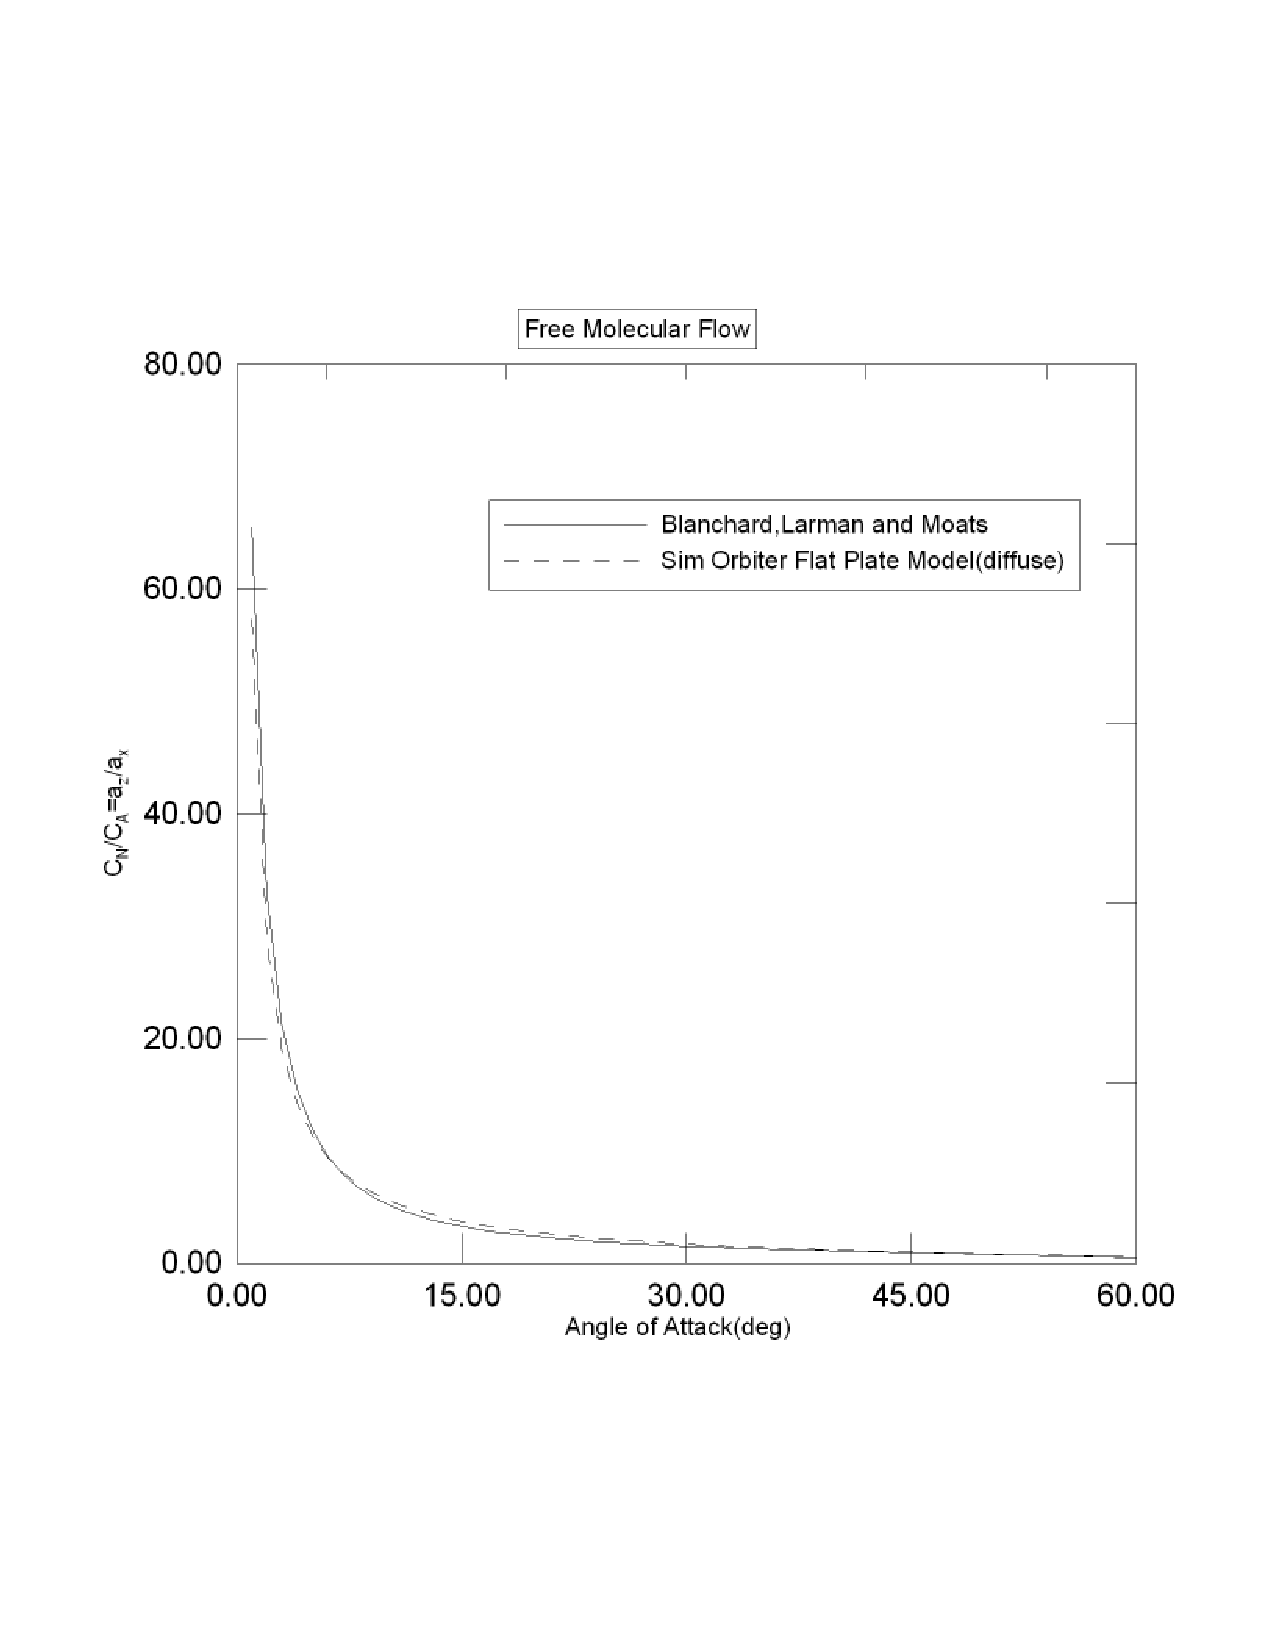
\includegraphics [width=7in]{figs/ratio.pdf}
\caption{Ratio of $C_n$ and $C_a$}
\label{fig:12}
\end{figure}
\clearpage
There is a small difference between the simulation and
the empirical data shown in figure~\ref{fig:13}.  The comparison between
the empirical and the simulation ratio differ by an average factor of 0.3.
Considering all the approximations and modeling errors that are involved
this is a good figure of merit for the flat plate representation of the
orbiter.  In fact a very good validation comparison using empirical data.
\begin{figure}[H]
\includegraphics [height=175mm]{figs/ratiodiff.jpg}
\caption{Difference simulated and empirical ratios}
\label{fig:13}
\end{figure}
\end{description}

\section{Metrics}
\subsection{Code Metrics}

Table~\ref{tab:coarse_metrics} presents coarse metrics on the
source files that comprise the model.

\input{coarse_metrics}

Table~\ref{tab:metrix_metrics} presents the extended cyclomatic
complexity
(ECC) of the methods defined in the model.
\input{metrix_metrics}


\section{Requirements Traceability}\label{sec:traceability}

\begin{longtable}[c]{||p{3in}|p{3in}|}
\caption{Requirements Traceability} \\[6pt]
\hline
{\bf Requirement} & {\bf Inspection and Testing} \\
\hline \hline
\endfirsthead
\hline
\endfoot
\caption[]{Requirements Traceability (continued)} \\[6pt]
\hline
{\bf Requirement} & {\bf Inspection and Testing} \\
\hline \hline
\endhead

\ref{reqt:toplevel} - Top-level Requirements &
  Inspection~\ref{inspect:TLI} \\
  \hline

\ref{reqt:aero_extension} - Aerodynamic Extensibility &
   Inspection~\ref{inspect:aero_extension} \\
\hline

\ref{reqt:AD} - Drag Data &
     Inspection \ref{inspect:math} \\
   & Inspection \ref{inspect:aerod} \\
   & Inspection \ref{inspect:FMF} \\
   \hline
\ref{reqt:drag} - Simple Drag &
     Inspection \ref{inspect:aerod} \\
   & Test \ref{test:sd} \\
   \hline
\ref{reqt:AFM} - Approximate Free Molecular &
     Inspection \ref{inspect:math} \\
                 Flow &
     Test \ref{test:amfs} \\
   \hline
\ref{reqt:AFM} - Approximate Free Molecular &
     Inspection \ref{inspect:math} \\
                 Flow &
     Test \ref{test:amfd} \\
   \hline
\ref{reqt:AFM} - Approximate Free Molecular &
     Inspection \ref{inspect:math} \\
                 Flow &
     Test \ref{test:amfm} \\
   \hline
\ref{reqt:FMF} - Free Molecular Flow &
     Inspection \ref{inspect:math} \\
   & Test \ref{test:mfs} \\
   \hline
\ref{reqt:AFM} - Approximate Free Molecular &
     Inspection \ref{inspect:math} \\
                 Flow &
     Test \ref{test:mfd} \\
   \hline
\ref{reqt:AFM} - Free Molecular Flow &
     Inspection \ref{inspect:math} \\
   & Test \ref{test:mfm} \\
   \hline
\ref{reqt:AS} - Aerodynamic Forces and Torques &
     Inspection \ref{inspect:math} \\
   & Test \ref{test:amfs}\\
   & Test \ref{test:amfd}\\
   & Test \ref{test:amfm}\\
   & Test \ref{test:mfs} \\
   & Test \ref{test:mfd}\\
   & Test \ref{test:mfm}\\
   & Test \ref{test:torque}\\
   & Test \ref{test:fmfo}
\end{longtable}


%%% or for a document with multiple parts make as many copies of Chapters.tex
%%% as you have parts and use this format
%\hyperdef{part}{part1}{\part{Part 1 Title}}\label{pt1:title}
%\include{aerodynamicsChapters1}
%\hyperdef{part}{part2}{\part{Part 2 Title}}\label{pt2:title}
%\include{aerodynamicsChapters2}
%%% etc.

%%%%%%%%%%%%%%%%%%%%%%%%%%%%%%%%%%%%%%%%%%%%%%%%%%%%%%%%%%%%%%%%%%%%%%%%%
% Bibliography
%%%%%%%%%%%%%%%%%%%%%%%%%%%%%%%%%%%%%%%%%%%%%%%%%%%%%%%%%%%%%%%%%%%%%%%%%
\newpage
\pdfbookmark{Bibliography}{bibliography}
\bibliography{dynenv,aerodynamics}
\bibliographystyle{plain}

%\pagebreak
%\appendix

\end{document}
